\documentclass{article}
\usepackage[utf8]{inputenc}

\title{Metodos Computacionales}
\author{Rafael Cordoba Lopez- 201630880 }
\date{November 2018}

\begin{document}

\maketitle

\section{Pregunta 1}
Parte de Git, se subió los commits respectivos para cada punto.
\section{Pregunta 2: PDE}
La seccion de ecuacion diferencial al final no compilo por problemas con las condiciones segmentation foult, el programa esta pero se tine dificultad en las condiciones. Se tienen las siguientes imagenes:
\begin{figure}
  \centering
    \includegraphics{condicionesfinales.pdf}
  \caption{Condiciones Finales}
  \label{fig:ejemplo1}
\end{figure}
\begin{figure}
  \centering
    \includegraphics{condicionesiniciales.pdf}
  \caption{Condiciones Iniciales}
  \label{fig:ejemplo2}
\end{figure}

\begin{figure}
  \centering
    \includegraphics{condicionesmitad.pdf}
  \caption{Condiciones Mitad}
  \label{fig:ejemplo3}
\end{figure}
En las graficas se observa que se tiene una gran diferencia segun las condiciones, en los bordes para el caso 3 oscila y para el caso 1 se mantienen fijos, ademas se ve la transmicion de calor sobre toda la superficie que se eleva en el diagrama 3d.
\section{Pregunta 3: ODE}
Se realizo el ejercico de Ecuaciones diferenciales ordinarias en dos dimensiones, se guardo en diferentes archivos por el tamaño de vectores y se obtuvo las siguientes graficas, como se espera se tiene las distancias de los angulos aumentan segun mayor velocidad en x e y, se observa lo siguietne:
\begin{figure}
  \centering
    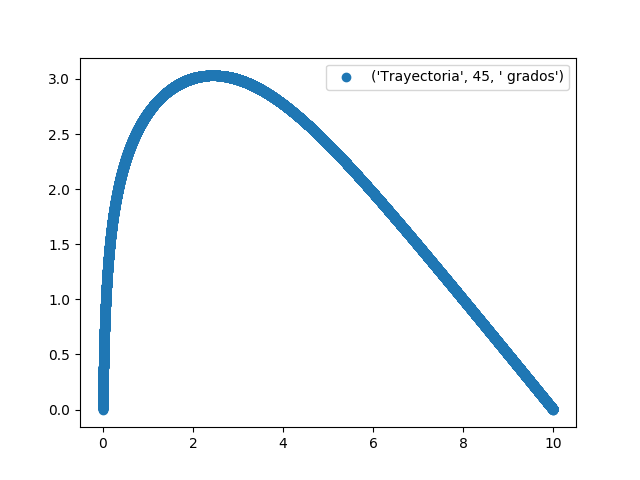
\includegraphics{('Trayectoria', 45, ' grados').png}
  \caption{Trayectoria 45}
  \label{fig:ejemplo1}
\end{figure}

\begin{figure}
  \centering
    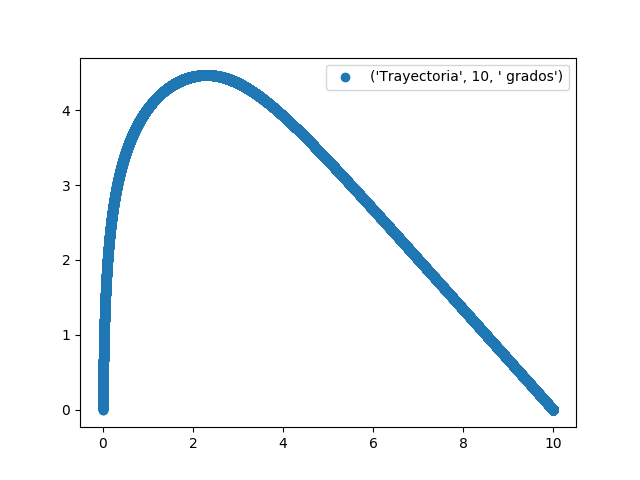
\includegraphics{('Trayectoria', 10, ' grados').png}
  \caption{Trayectoria 10}
  \label{fig:ejemplo1}
\end{figure}
\begin{figure}
  \centering
    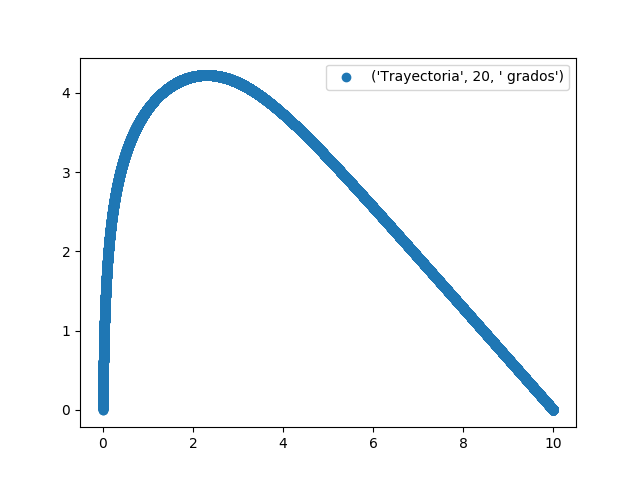
\includegraphics{('Trayectoria', 20, ' grados').png}
  \caption{Trayectoria 20}
  \label{fig:ejemplo1}
\end{figure}
\begin{figure}
  \centering
    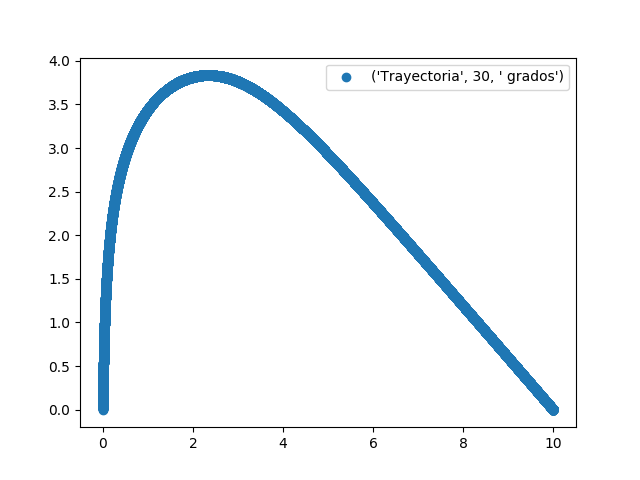
\includegraphics{('Trayectoria', 30, ' grados').png}
  \caption{Trayectoria 30}
  \label{fig:ejemplo1}
\end{figure}

\begin{figure}
  \centering
    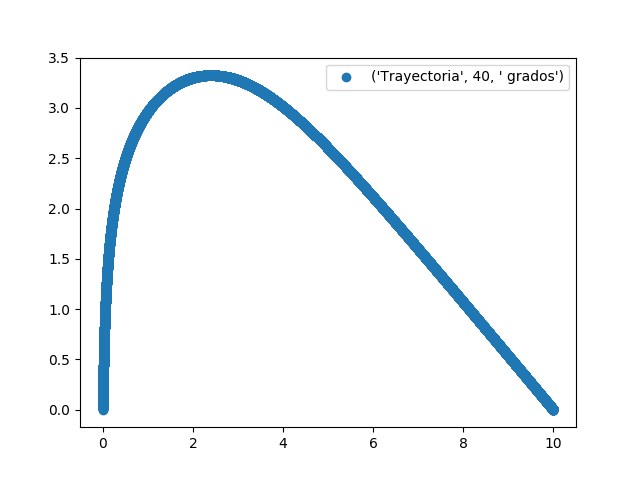
\includegraphics{('Trayectoria', 40, ' grados').png}
  \caption{Trayectoria 40}
  \label{fig:ejemplo1}
\end{figure}
\begin{figure}
  \centering
    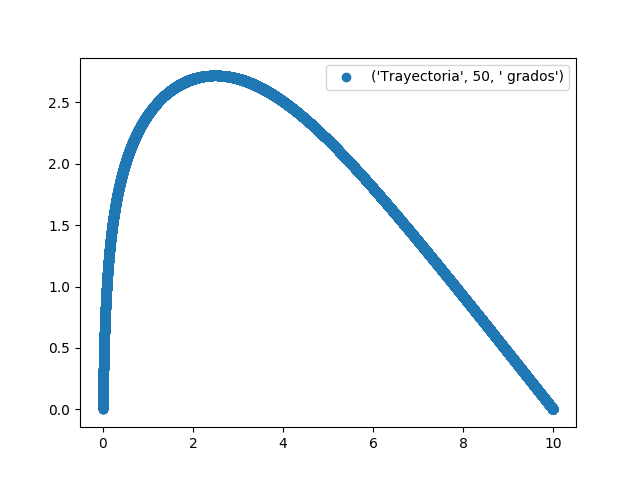
\includegraphics{('Trayectoria', 50, ' grados').png}
  \caption{Trayectoria 50}
  \label{fig:ejemplo1}
\end{figure}
\begin{figure}
  \centering
    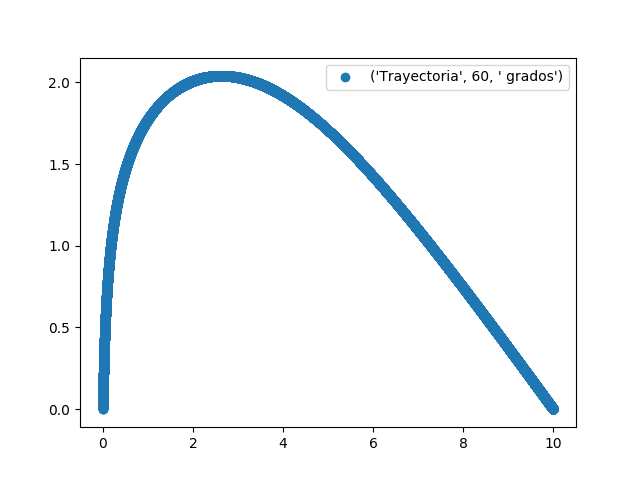
\includegraphics{('Trayectoria', 60, ' grados').png}
  \caption{Trayectoria 60}
  \label{fig:ejemplo1}
\end{figure}
\begin{figure}
  \centering
    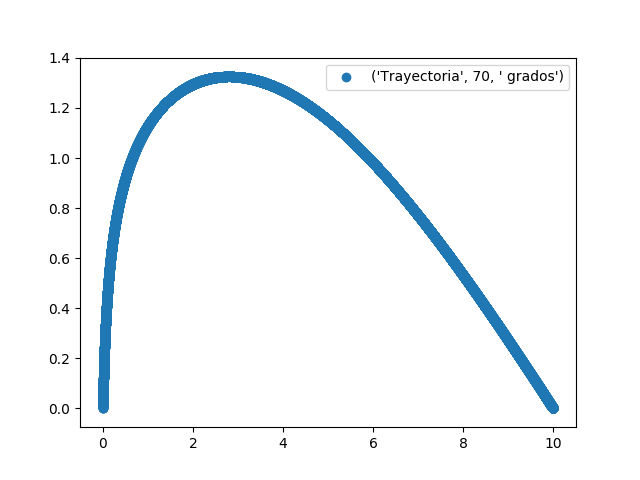
\includegraphics{('Trayectoria', 70, ' grados').png}
  \caption{Trayectoria 70}
  \label{fig:ejemplo1}
\end{figure}
\section{Pregunta 4}
Se creo este archivo mediante el make file.
\end{document}
